\chapter{Techniques used}\label{Methodology}

In this section, the process of learning arguments is discussed in its entirety.

\section{Discretization Techniques}\label{Section_Discretization_Techniques}

With the exception of decision trees, the rule-mining algorithms in this project cannot be trained on continuous data. Therefore, in order to apply the rule-mining algorithms to datasets, we must rely on data discretization techniques to preprocess the data before mining the rules. In the data, every numerical feature of a dataset is considered to be continuous.

\subsection*{Equal-Width Binning}
This algorithm is a comparatively simple binning technique. Here, the range spanned by the smallest and largest value of a feature (referred to as $min$ and $max$ respectively,) is divided into a number of bins $k$, where each of these bins have size $\frac{max-min}{k}$. To discretize, values are assigned to the respective bin they fall into.

% JONAS: "Instead of talking about general flaws of the algorithm, we will focus on the performance of the algorithm in our experiments."

% This approach is easy to implement and not computationally expensive. However, there are some notable flaws: This algorithm assumes that each cluster has the same diameter, and it is prone to outliers due to reliance on minimum and maximum values of a feature. 

\subsection*{Equal-Depth Binning}
Equal-depth or equal-frequency binning is another simple discretization approach. Here, values are assigned to one of $k$ bins, such that each bin approximately holds the same number of instances. This is done by sorting the values of the feature and assigning $\frac{n}{k}$ of the sorted instances into each bin, where $n$ is the number of total values.

\subsection*{Clustering approaches}

To discretize more complex features in the data, clustering approaches are considered. Here, values of a given feature in the data are clustered, and replaced by the discretized value. In the dataset, clusters are represented as ranges, where each cluster is described by its smallest and largest value. By the nature of the given clustering algorithms, these ranges do not overlap.

\subsubsection*{K-Means Clustering}
K-Means \citep{LeastSquareLloyd} is based on the idea of centroids, which are points in the centre of the cluster. Here, $k$ centroids are initialized randomly, and the instances are assigned to the cluster whose centroid is closest. Then, the centroids are moved to the mean of the cluster, and the instances are assigned to their new cluster. The algorithm converges when the movement of centroids is below a certain threshold.

% One flaw of this algorithm is that it is sensitive to outliers due to reliance of mean values. It is also highly dependant on the random initialization. Additionally, this algorithm assumes that every cluster has a similar diameter, which may not be true for some datasets.

\subsubsection*{DBSCAN Clustering}

DBSCAN  by \citet{DBSCANPaper} considers clusters to be regions of high density. For each instance, the algorithm counts the number of instances within a distance $\epsilon$, also called the instance's $\epsilon$-neighbourhood. If this number of neighbours of an instance surpasses a given threshold, the instance is considered to be a core instance, an instance within a dense region. The neighbours of this core instance are considered to be in the same cluster, where some neighbours may also be core instances themselves. Therefore, a cluster consists of a multitude of core instances. 
% This algorithm can fail in identifying clusters if density varies for clusters, or for spare regions of a feature.

\subsection*{Cluster Optimization}

The aforementioned clustering algorithms all provide parameters that can be tuned in order to find  clusters representing the data correctly. In this project, the silhouette score introduced by \citet{ROUSSEEUW198753} has been utilized to provide a metric for accuracy of clusters. This score computes the mean silhouette coefficient of all samples (given by equation \ref{Silhouette_Coefficient}).

\begin{equation}
\label{Silhouette_Coefficient}
    silhouette\_ score = \frac{b - a}{\max(a, b)}
\end{equation}

\noindent In equation \ref{Silhouette_Coefficient}, $a$ denotes the mean distance to the other instances in the same cluster (intra-cluster distance) and $b$ denotes the minimal distance to another instance that is not part of the same cluster (nearest-cluster distance).

Clusters are optimized by exhaustive search this project, i.e., every combination of parameters is tested using the silhouette score, before returning the parameters resulting in the highest score.

\subsection*{Discretization of prediction data}

Once the data is discretized and rule-mining is performed, rules have to be applicable to the original, continuous features in order to predict the outcome. While discretized values are represented as ranges of the minimum and maximum value of the given bin or cluster, not all values to be predicted may fall into these given bins. Therefore, to discretize the new values, distances are measured to each of the boundaries of a given bin. Then, the value is assigned to the bin with the smallest distance for either boundary.

\section{Learning arguments}\label{Section_Learning_Arguments}

% Skip this for proofreading for now, will rewrite most of it

We have implemented four different algorithms for learning arguments from data. The first two algorithms are devised by ourselves, the third one is implemented by ourselves according to the high-level description in \cite{johnstonInductionDefeasibleLogic2003}, and the fourth one is based on the open-source library \textit{scikit-learn} \citep{pedregosa2011scikit}.

\subsection{Naive search}

The naive search algorithm follows the generate-and-test paradigm: Firstly, all possible arguments are generated, and secondly they are tested whether they are conclusive, presumptively valid, or coherent. The generation of all possible arguments is very inefficient: For a dataset with $k$ columns and $n$ bins per column, the space of all sensible combinations of literals is of size $n^k$. The algorithm is therefore only suitable for very small datasets such as the toy examples in \autoref{appendix-notebook}.

An important feature of the naive search is the postprocessing of the rules, consisting of (1.) filtering and (2.) merging:

\begin{enumerate}
    \item The filtering step is necessary for removing irrelevant rules. For example, when there are two arguments $a \rightsquigarrow d$ and $a \land b \land c \rightsquigarrow d$, then the second argument is more specific than the first argument and therefore only relevant if there is another relevant argument, such as $a \land b \rightsquigarrow \neg c$, to which it is an exception. Generally speaking, an argument A is relevant if there is no less specific argument to A, or if A is an exception to a relevant argument. We say that an argument $(P_1, c_1)$ is more specific than another argument $(P_2, c_2)$, if its premises $P_1$ are a proper superset of the premises $P_2$ of the other argument. 
    \item During the argument generation, we only generate arguments with a conclusion of a single literal. We reduce the number of arguments for legibility by merging together any arguments $(P_1, c_1)$, ..., ($P_m, c_m)$ that have the same premises $P_1=...=P_m$ to a single argument $(P_1= ...= P_2, \{c_1\} \cup ... \cup \{c_m\})$ with multiple conclusions.
\end{enumerate}

\label{sec:pruned-search-meth}
\subsection{Pruned search}

\begin{figure}[htb]
        \centering
        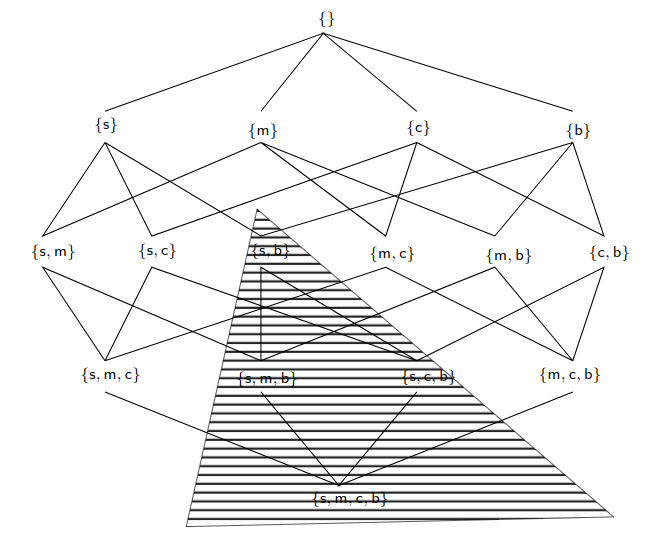
\includegraphics[width=0.6\textwidth]{images/pruning.png}
        \caption{\textit{Pruning specializations.} From \citet[p.~52]{deraedtLogicalRelationalLearning2008}. All $2^n$ subsets of $\{s, m, c, b\}$ are systematically searched, starting from the most general set at the top. Knowing that the set $\{s, b\}$ is infrequent allows us to prune all its specializations, which is a lot. }
        \label{fig:pruning}
\end{figure}

\label{pruned-search}
\begin{algorithm}
\caption{Pruned search.}
\For{each literal p}{
    search(premises=$\varnothing$, target=p, depth, max\_size)\\
    remove arguments that are more specific to another argument \\
    \hspace{1cm}but are no exception to another argument\\
    merge arguments with the same premises
}
$\vspace{0.5cm}$
\Function{search}{premises, target, depth, max\_size}: \\
candidate\_arguments := $\{(\text{premises} \cup \{p\}, \text{target}) | p \in \text{literals}\}$ \\
determine and save which candidate arguments are \\
\hspace{1cm}conclusive, presumptively valid, and coherent given the data \\
\For{each presumptively valid argument (P, c)}{
    search for exceptions: \\
    \For{each literal p about the same fact as c, except c itself}{
        \If{depth $> 0$}{
            search(premises=P, target=p, depth - 1, max\_size)\\
            save the results
        }
    }
}
\For{each $(P_1, P_2), \text{where}\\
    \hspace{2.5cm} (P_1, c_1) \in \text{candidate\_arguments}, \\
    \hspace{2.5cm} (P_2, c_2) \in \text{candidate\_arguments}, \\
    \hspace{2.5cm} |P_1 \cap P_2| = |\text{premises}|,\\
    \hspace{2.5cm}|\text{premises}| < \text{max\_size}$ \\
}{
    search for more specific arguments: \\
    search(premises=$P_1 \cup P_2$, target=target, depth, max\_size) \\
    save the results
}
\EndFunction
\end{algorithm}

\noindent The pruned search algorithm improves the runtime by pruning the search space in a systematic way. This technique is known from frequent pattern mining (and its application to association rule mining; see \cite{agrawalFastAlgorithmsMining1994}), and is described in the context of logical learning in \cite{deraedtLogicalRelationalLearning2008}. The idea is to identify a quality criterion, for which the following is true: If a set fulfils the quality criterion, all its subsets must also fulfil the quality criterion. (Alternatively: If a set fulfils the quality criterion, all its \textit{super}sets must also fulfil the quality criterion; this an be visualized by "flipping" the search space or the direction of the search). For example, in the context of frequent pattern mining, if a set is frequent, then all its subsets must also be frequent. The principle of pruning the search space is visualized in \autoref{fig:pruning}.

This raises the issue of the selection of a suitable quality criterion for pruning the search space in our application of learning arguments. We find two quality criteria: 

\begin{enumerate}
    \item \textit{If an argument $(P, c)$ is conclusive, then all coherent arguments $(P', c)$ must also be conclusive, for all $P'$ that are a superset of $P$.} 
    % (Proof: The argument $(P, c)$ is conclusive iff $c$ holds in all cases where $P$ holds. ...
    % However, the arguments $(P', c)$ need not be coherent, and thus in an additional step the coherence ... not sure!
    \item \textit{If an argument $(P, c)$ is coherent, then all arguments $(P', c)$ must also be coherent, for all $P'$ that are a subset of $P$.}
\end{enumerate}

The most important part of the learning algorithm in terms of efficiency is the learning of presumptively valid argument: They are relevant for a prediction, and there are equally many or (usually) many more  presumptively valid arguments than conclusive arguments. So it would be nice if we could find a quality criterion for learning presumptively valid arguments. Unfortunately, presumptive validity, unlike conclusivity or coherence, is not itself a quality criterion: 

\textit{Proof by contradiction:} Consider the case model $ (1, \{a,b,c,d\})\}, (2, \{a, b, \neg c, \neg d\}), \{(3, \{a, \neg b, \neg c, d\})$. A higher number denotes a higher priority of the case. $(\{a, b\}, \neg d)$ is a presumptively valid argument in the case model, since the case with the highest priority where its premises hold is the second case; and its conclusion also holds in the second case. \\
Assume that presumptive validity is a quality criterion. So, either (a) if an argument $(P, c)$ is presumptively valid, then all arguments $(P', c)$ must also be presumptively valid, for all $P'$ that are a subset of $P$; or (b) if an argument $(P, c)$ is presumptively valid, then all arguments $(P', c)$ must also be presumptively valid, for all $P'$ that are a superset of $P$. Consider (a): Then $(\{a\}, \neg d)$ must also be presumptively valid. But the most likely case where the premises hold is the third case, and there its conclusion does not hold, so it is not presumptively valid, contradiction. Consider (b): Then $(\{a, b, c\}, \neg d)$ must also be presumptively valid, but the most likely case where its premises hold is the first case, and its conclusion does not hold there, so it is not presumptively valid, contradiction. Contradiction in (a) and (b), and either (a) or (b), so overall contradiction.\\
Thus, presumptive validity is not a quality criterion, no matter in what direction we would like to prune the search space.\square

We cannot use presumptive validity itself as a quality criterion for pruning the search space, but we can at least use a condition for presumptive validity: Coherence. \autoref{pruned-search} shows our algorithm, which uses coherence to prune the search space. We separately start a search for each literal (each combination of column and bin), looking for arguments with this literal as a conclusion. After search is completed, we filter and merge the resulting arguments in the same way as described for the naive search algorithm. At each search step $i$ we consider arguments with $i$ premises (that is, a premise size of $i$). 

At the end of the search step we gather all coherent arguments of the step, and check all combinations of these arguments whether their premises are different in exactly two literals. The reason is: If they are different in two literals, we can take the union of the premises as a new premise of size $i+1$, and we know that many subsets of this premise lead to a coherent argument. Consider, for example, two premises $\{a,b,c,d\}$ and $\{b,c,d,e\}$: The union is $\{a,b,c,d,e\}$ with size $n=5$. Enumeration shows that $2^n-2^{n-2} = 24$ of its subsets are also subsets of at least one of the two premises of which we already know that they are coherent. It is thus much more likely for the new premise to also be coherent than it would be for an arbitrary premise. 

This principle of combining small sets fulfilling the quality criterion into larger sets likely to fulfil the quality criterion is known from the Apriori algorithm (see \cite{tanIntroductionDataMining2014}). There, it makes the algorithm suitable for big datasets. Here, because coherence is only a condition but not the same as presumptive validity (which we are looking for), it at least makes the algorithm efficient enough for the medium-sized datasets we use.

\label{hero-meth}
\subsection{HeRO algorithm}
% HeRO algorithm is a kind of method for computing square roots 

\begin{figure}[htb]
        \centering
        
\includegraphics[width=0.4\textwidth]{images/hero.jpg}
        \caption{\textit{Hero algorithm.} \textcopyright Curvabezier, dreamstime.com}
        \label{fig:hero}
\end{figure}

The HeRO algorithm has been devised by \cite{johnstonAlgorithmInductionDefeasible2003}, and the research behind it, like \cite{verheijProofProbabilities2017}, is also originally targeted towards the legal domain \citep{johnstonInductionDefeasibleLogic2003}. It does not primarily perform a systematic search, but rather an incremental search: At each step, it considers which argument would be most valuable to be added to the theory in order to increase the accuracy the most; and then it adds the most valuable argument to the theory and asks the question again, until there is no more argument that can increase the accuracy. 

The algorithm builds up a totally ordered set of arguments, and at every step it considers all positions (before, after, or between the existing arguments) for adding the next argument. For determining the most valuable argument (and its most valuable position), the criterion of \textit{information gain}, that is increase in accuracy on the training set, is used. Similar to the pruned search algorithm presented above, the HeRO algorithm also starts by considering simple arguments and then in some cases also considers arguments where the premises are more specific. The mechanism for deciding whether more specific premises should also be considered uses the criterion of \textit{maximum information gain}. The maximum information gain of an argument is the highest information gain that can be achieved by any argument that is more specific. This is equivalent to the information gain that would be achieved by adding an argument that correctly predicted all the rows where the premises hold. 

Formulas for information gain and maximum information gain and a high-level pseudocode algorithm are provided in \cite{johnstonAlgorithmInductionDefeasible2003}. The authors also briefly mention a few optimization techniques, which we have not implemented. There is no public implementation of the HeRO algorithm, so we are the first to provide a such. Since the description by the authors is on a high level only, our algorithm, apart from the optimizations, may also differ from the original algorithm in other minor ways. 

\label{dectrees-meth}
\subsection{Decision trees}

To classify by building tree models, the open-source library \textit{scikit-learn} \citep{pedregosa2011scikit} is used. This implementation utilizes the CART \citep{DecTreePaper} algorithm. Here, the tree is built choosing a feature $k$ and a threshold $t_k$ by using a cost function measuring the purity of the subsets produced by the split. In this project, this is measured by the Gini impurity introduced by \citet{DecTreePaper}. Once the split has been made, the algorithm iteratively splits the subsets further, until a given maximum depth is reached, or no split reducing impurity can be found.

In a decision tree, the nodes at the bottom of the tree are referred to as leaf nodes, or internal nodes. Trees can be converted into decision rules, where each leaf node is associated with one rule. Here, the path traversed through the decision tree represents the premises that must hold for the conclusion at the child node.

\subsubsection*{Hyperparameter Tuning of Decision Trees}\label{Section_Bayesian_Optimization}

To maximize performance of the decision tree algorithm, various hyperparameters can be tuned. In this project, this is done via Bayesian Optimization \citep{BayesOptPaper} utilizing the \textit{scikit-optimize} package \citep{skopt}. This algorithm samples points to construct an interpolation function, also called posterior function. This function represents the objective function (which, in this case, is a function measuring the accuracy of the tree with its parameters as inputs). New points are found using an acquisition function, which balances exploration and exploitation by calculating uncertainty in the posterior function. These query points are then used to update the posterior function. After a given number of iterations, the algorithm converges, returning an estimate of the optimal parameters by using the posterior function.